% Provenance (never printed): see sources/outline_sources.md (Year 1: insolation with
% latitude and season, the radiative surplus and deficit, meridional heat transport by
% the atmosphere and the ocean, latent heat). Exercise and problem values in the Book 3
% scratch calculator calc/ch27.py; figures from figdata/bachelor-1/insolation.py (Kepler
% orbit of _solar.py) and energy_balance.py (NCEP-NCAR Reanalysis 1, long-term means
% 1991-2020, datasets bachelor-1-ncep-*).
% Physics owns the inverse-square law, the black body and the Stefan-Boltzmann law, the
% seasons and latent heat (recalled). Book 2 (g10) gave the quarter of the solar constant,
% the global budget diagram and its closure, latent and sensible heat in words, the
% annual-mean insolation curve and the poleward transport in words: re-founded here with
% derivations and data. Ch. 1 gave the instantaneous insolation, the declination and the
% rising and setting of the Sun.
\chapter{الإشعاع ونقل الحرارة}\label{ch:b1:radiation-heat-transport}

من مسافة مليون ميل، يبدو الوجه المضاء من الأرض قرصًا من بحر أزرق، وأرض بنّية، وسحاب أبيض. يسقط ضوء الشمس بأكبر استقامة على وسط القرص، قرب المدارات، ويمرّ مماسًا لحوافه؛ فالمناطق المدارية تمتصّ طاقة أكثر بكثير من المناطق القطبية. ومع ذلك لا تزداد المناطق المدارية حرارة عامًا بعد عام، ولا تزداد القطبان برودة. تحمل الرياح وتيارات المحيط الفائض نحو القطبين، وهو عدّة بيتاوات. يقيس هذا الفصل الحدود الثلاثة لهذا التوازن: ضوء الشمس الذي يتلقّاه كل خطّ عرض، والجزء الذي يحتفظ به وما يُرسله من أشعة تحت حمراء إلى الفضاء، والنقل الذي يسدّ الفرق. ويسير جزء كبير من النقل في شكل غير مرئي، هو بخار الماء، الذي تنطلق حرارته الكامنة حيثما يتكثّف مطرًا.
% ledger: commons:epic-earth, trenberth:transport

\begin{omfigure}
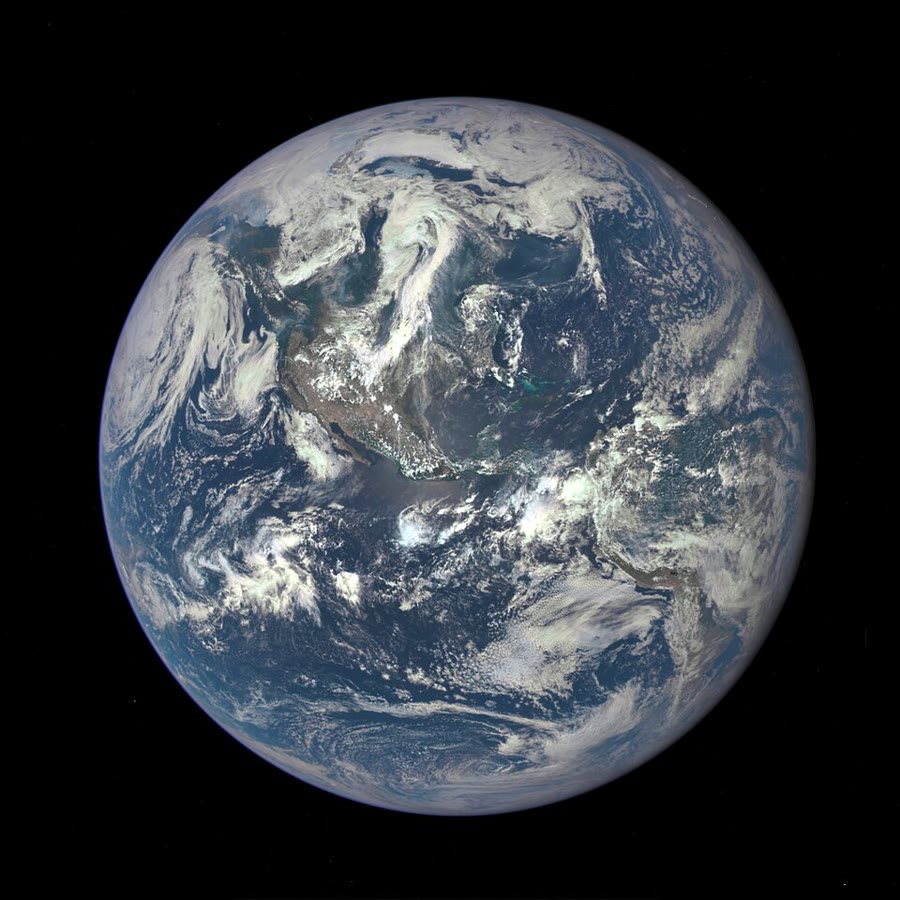
\includegraphics[width=0.55\linewidth]{images/book3/b1-epic-earth.jpg}

{\small الجانب المضاء كاملًا من الأرض، مُصوَّرًا في 6 يوليو 2015 بكاميرا على مرصد المناخ في الفضاء العميق، على بعد مليون ميل؛ وتقع أمريكا الشمالية والوسطى في الوسط، مع البحار الضحلة الفيروزية في الكاريبي. وبعد أسبوعين من انقلاب يونيو يُضاء القطب الشمالي، في الأعلى، طوال الوقت. تعكس السحب اللامعة كثيرًا من الضوء الذي يصل إليها؛ والصبغة المائلة إلى الزرقة ضوء الشمس المبعثر بجزيئات الهواء. (NASA Goddard Space Flight Center, ملك عام، عبر Wikimedia Commons.)}
\label{fig:b1:radiation-heat-transport:epic}
\end{omfigure}
% ledger: commons:epic-earth (polar day: figdata/bachelor-1/insolation.py)

\begin{recall}
\Cref{ch:b1:spherical-astronomy} عرّف الإشعاع الشمسي، أي قدرة ضوء الشمس المستقبلة على كل متر مربّع من سطح أفقي عند أعلى الغلاف الجوي، $I = S_0(a/r)^2\sin h_\odot$ ما دامت الشمس فوق الأفق، مع $S_0 = \qty{1361}{W.m^{-2}}$ عند المسافة المتوسطة $a$؛ وأعطى \omterm{def:b1:spherical-astronomy:horizontal}{ارتفاع الشمس} من زاويتها الساعية $H$، وميلها $\delta$ وخطّ عرضها $\varphi$، $\sin h_\odot = \sin\varphi\sin\delta + \cos\varphi\cos\delta\cos H$؛ \omterm{def:b1:spherical-astronomy:equatorial}{والزاوية الساعية} $H_0$ للغروب، $\cos H_0 = -\tan\varphi\tan\delta$ (\cref{prop:b1:spherical-astronomy:rising}). و\Cref{ch:b1:comparative-planetology} عرّف \omterm{def:b1:comparative-planetology:albedo}{ألبيدو بوند} الكوكب ودرجة حرارته التوازنية. وتعطي مجلّدات الفيزياء قانون التربيع العكسي للضوء، وإشعاع الجسم الأسود، $\sigma T^4$ لكل متر مربّع مع $\sigma = \qty{5.670e-8}{W.m^{-2}.K^{-4}}$ (ستيفان--بولتزمان)، والحرارة الكامنة لتغيّر الحالة. وأظهر الكتاب~2 أن الأرض تعترض في المتوسط ربع الثابت الشمسي، ورسم ميزانية الطاقة العامة للأرض وتحقّق من توازنها، ووصف نقل الحرارة نحو القطبين بالكلام.
% ledger: earth:TSI, const:sigma, ipcc:budget-toa
\end{recall}

\section{الإشعاع الشمسي حسب خطّ العرض والفصل}\label{sec:b1:radiation-heat-transport:insolation}

يتغيّر الإشعاع الشمسي اللحظي من دقيقة إلى أخرى مع عبور الشمس السماء. أما المناخ فيهمّه مجموعه على مدار اليوم.

\begin{definition}[متوسط الإشعاع اليومي]\label{def:b1:radiation-heat-transport:daily-insolation}
\emph{متوسط الإشعاع اليومي}\index{متوسط الإشعاع اليومي} $\bar Q$ عند خطّ عرض معيّن في يوم معيّن هو الإشعاع الشمسي اللحظي متوسَّطًا على ساعات اليوم الأربع والعشرين، مع احتساب الليل، \omterm{def:b1:spherical-astronomy:equatorial}{والميل الشمسي} وبعد الشمس ثابتان عند قيمتيهما لذلك اليوم. وهو قدرة لكل متر مربّع من سطح أفقي عند أعلى الغلاف الجوي، بوحدة \unit{W.m^{-2}}.
\end{definition}

تثبيت $\delta$ و$r$ ليومٍ واحد غير ضارّ: \omterm{def:b1:spherical-astronomy:equatorial}{فالميل الشمسي} يتغيّر بما لا يزيد على \ang{0.4} في اليوم، والمسافة بأقلّ من \qty{0.03}{\percent}.
% ledger: earth:obliquity, earth:ecc (computed in figdata/bachelor-1/insolation.py)

\begin{theorem}[متوسط الإشعاع اليومي]\label{thm:b1:radiation-heat-transport:daily}
عند خطّ العرض $\varphi$، في يوم يكون فيه \omterm{def:b1:spherical-astronomy:equatorial}{ميل الشمس} الميل $\delta$ وبعدها $r$،
\[
  \bar Q = \frac{S_0}{\pi}\left(\frac{a}{r}\right)^{2}
  \bigl(h_0\sin\varphi\sin\delta + \cos\varphi\cos\delta\sin h_0\bigr),
\]
حيث $h_0 \in [0, \pi]$ هي \omterm{def:b1:spherical-astronomy:equatorial}{الزاوية الساعية} للغروب بالراديان: $\cos h_0 =
-\tan\varphi\tan\delta$ حين تكون $|\tan\varphi\tan\delta| \le 1$؛ و$h_0 = \pi$ في النهار القطبي ($\tan\varphi\tan\delta > 1$)؛ و$h_0 = 0$، و$\bar Q = 0$، في الليل القطبي
($\tan\varphi\tan\delta < -1$).
\end{theorem}

\begin{proof}
تتقدّم \omterm{def:b1:spherical-astronomy:equatorial}{الزاوية الساعية} $H$ بانتظام عبر $2\pi$ في اليوم، فالمتوسط على اليوم هو المتوسط على $H \in [-\pi, \pi]$. والشمس فوق الأفق عندما $-h_0 < H < h_0$، حيث $\sin h_\odot > 0$، والإشعاع الشمسي اللحظي منعدم في غير ذلك. ومن ثمّ
\[
  \bar Q = \frac{1}{2\pi}\int_{-h_0}^{h_0} S_0\left(\frac{a}{r}\right)^{2}
  \bigl(\sin\varphi\sin\delta + \cos\varphi\cos\delta\cos H\bigr)\,\mathrm dH ,
\]
أي $(S_0/2\pi)(a/r)^2\bigl(2h_0\sin\varphi\sin\delta +
2\cos\varphi\cos\delta\sin h_0\bigr)$.
وتأتي الحدود من \cref{prop:b1:spherical-astronomy:rising}: يكون الارتفاع صفرًا حين $\cos H = -\tan\varphi\tan\delta$. فإن تجاوز هذا العدد 1 في القيمة المطلقة لم تعبر الشمس الأفق أبدًا: حين $\tan\varphi\tan\delta > 1$، تكون الدالة المكامَلة موجبة لكل $H$، ويمتدّ التكامل على اليوم كله، $h_0 = \pi$؛ وحين $\tan\varphi\tan\delta < -1$، تكون سالبة لكل $H$، ولا تشرق الشمس أبدًا.
\end{proof}

تستحقّ حالتان خاصّتان أن تُحفظا عن ظهر قلب. عند خطّ الاستواء، $\varphi = 0$ و
$h_0 = \pi/2$ مهما كان الفصل:
\[
  \bar Q_\text{الاستواء} = \frac{S_0}{\pi}\left(\frac{a}{r}\right)^{2}\cos\delta ,
\]
وهو أكبر ما يكون عند الاعتدالين، و$S_0/\pi = \qty{433.2}{W.m^{-2}}$ عند المسافة المتوسطة. وعند قطب في صيفه، $h_0 = \pi$ و$\varphi = \pi/2$: $\bar Q_\text{القطب} =
S_0(a/r)^2\sin\delta$، فالشمس تدور في السماء على ارتفاع ثابت يساوي الميل.
% ledger: earth:TSI

\begin{proposition}[الصيف القطبي]\label{prop:b1:radiation-heat-transport:polar-summer}
في يوم يكون فيه الميل $\delta > 0$، يتجاوز \omterm{def:b1:radiation-heat-transport:daily-insolation}{متوسط الإشعاع اليومي} عند القطب الشمالي نظيره عند خطّ الاستواء إذا وفقط إذا كان $\pi\tan\delta > 1$، أي $\delta >
\ang{17.66}$. وعند انقلاب يونيو، $\delta = \ang{23.44}$، والنسبة $\pi\tan
\delta = 1.362$.
\end{proposition}

\begin{proof}
تشترك الحالتان الخاصتان أعلاه في العامل $(S_0/\pi)(a/r)^2$؛ ونسبتهما $\pi\sin\delta/\cos\delta = \pi\tan\delta$، وهي أكبر من 1 حين يكون $\tan\delta >
1/\pi$، أي $\delta > \arctan(1/\pi) = \ang{17.66}$. وبميل المحور،
$\pi\tan\ang{23.44} = 1.362$.
\end{proof}
% ledger: earth:obliquity

بمدار الأرض، يقع انقلاب يونيو قرب الأوج، $(a/r)^2 = 0.968$: فيتلقّى القطب الشمالي \qty{524}{W.m^{-2}} متوسطًا يوميًّا، وخطّ الاستواء \qty{385}{W.m^{-2}}. وبعد ستّة أشهر يتلقّى القطب الجنوبي، قرب الحضيض، \qty{559}{W.m^{-2}}، أي \qty{6.7}{\percent} أكثر مما تلقّاه القطب الشمالي في صيفه: والنسبة هي بالضبط نسبة قيمتي $(a/r)^2$. يُظهر الشكل أدناه $\bar Q$ على مدار سنة كاملة. وتقع القمم عند القطبين في الانقلابين؛ والأسافين الداكنة هي الليالي القطبية، يحدّها خطّ العرض $\ang{90} -
|\delta|$؛ أمّا نقطة تحت الشمس، حيث تمرّ الشمس فوق الرأس عند الظهيرة، فتتحرّك بين المدارين مع الميل.
% ledger: earth:TSI, earth:ecc, earth:obliquity, nasa:earth-perihelion-longitude, usno:seasons-2026 (computed in figdata/bachelor-1/insolation.py)

\begin{omfigure}
\begin{tikzpicture}
\begin{axis}[omrecord, width=0.8\linewidth, height=6.4cm, view={0}{90},
  xmin=0, xmax=365, ymin=-90, ymax=90, xlabel={اليوم من السنة (من 1 يناير)},
  ylabel={خطّ العرض (\unit{\degree})}, xtick={0,60,...,360}, ytick={-90,-60,...,90},
  colormap/viridis, colorbar, point meta min=0, point meta max=560,
  colorbar style={ylabel={$\bar Q$ (\unit{W.m^{-2}})}, ytick={0,100,...,500}, width=0.3cm},
  axis on top, grid=none]
% figdata/bachelor-1/insolation.py; ledger: earth:TSI, earth:ecc, earth:obliquity, nasa:earth-perihelion-longitude, usno:tropical-year, usno:seasons-2026
\addplot3[surf, shader=interp, mesh/ordering=y varies, mesh/rows=73]
  table[x=day, y=lat, z=Q] {figdata/out/bachelor-1-insolation-grid.dat};
\addplot3[white, dashed, line width=0.8pt] table[x=day, y=decl, z expr=600] {figdata/out/bachelor-1-insolation-sun.dat};
\addplot3[white, line width=0.6pt, unbounded coords=jump] table[x=day, y=night_n, z expr=600] {figdata/out/bachelor-1-insolation-sun.dat};
\addplot3[white, line width=0.6pt, unbounded coords=jump] table[x=day, y=night_s, z expr=600] {figdata/out/bachelor-1-insolation-sun.dat};
\node[font=\scriptsize, text=white] at (axis cs:28,81,700) {ليل قطبي};
\node[font=\scriptsize, text=white] at (axis cs:172,-81,700) {ليل قطبي};
\node[font=\scriptsize, text=white, anchor=south] at (axis cs:172,26,700) {خطّ العرض تحت الشمس};
\end{axis}
\end{tikzpicture}

{\small \omterm{def:b1:radiation-heat-transport:daily-insolation}{متوسط الإشعاع اليومي} عند أعلى الغلاف الجوي مقابل يوم السنة وخطّ العرض، من \cref{thm:b1:radiation-heat-transport:daily} مع $S_0 = \qty{1361}{W.m^{-2}}$ ومدار الأرض. متقطّع: خطّ العرض تحت الشمس، المساوي للميل الشمسي؛ متصل: حافّتا الليالي القطبية. ويتلقّى القطبان الصيفيان أكثر من أيّ مكان آخر على الأرض؛ والصيف الجنوبي، قرب الحضيض، هو الأشدّ إشراقًا من الاثنين.}
\label{fig:b1:radiation-heat-transport:matrix}
\end{omfigure}
% ledger: earth:TSI, earth:ecc, earth:obliquity, nasa:earth-perihelion-longitude, usno:seasons-2026

بتوسيط $\bar Q$ على السنة نحصل على الإشعاع الشمسي السنوي المتوسط لكل خطّ عرض
(الشكل أدناه): \qty{415.6}{W.m^{-2}} عند خطّ الاستواء، و\qty{328.3}{W.m^{-2}} عند
\ang{40}، و\qty{172.4}{W.m^{-2}} عند كل قطب. فالصيف القطبي شديد لكن الشتاء القطبي مظلم، وعلى مدار السنة يتلقّى خطّ الاستواء \num{2.41} مرّة ما يتلقّاه القطب. والمنحنى نفسه في النصفين، مع أن الصيف الجنوبي أشدّ إشراقًا؛ و\cref{exo:b1:radiation-heat-transport:10} يبيّن السبب.
% ledger: earth:TSI, earth:ecc, earth:obliquity (computed in figdata/bachelor-1/insolation.py)

\begin{omfigure}
\begin{tikzpicture}
\begin{axis}[omrecord, width=0.8\linewidth, height=5.6cm, xmin=-90, xmax=90, ymin=0, ymax=600,
  xlabel={خطّ العرض (\unit{\degree})}, ylabel={$\bar Q$ (\unit{W.m^{-2}})},
  xtick={-90,-60,...,90}, ytick={0,100,...,600}]
% figdata/bachelor-1/insolation.py; ledger: earth:TSI, earth:ecc, earth:obliquity, nasa:earth-perihelion-longitude
\addplot[omThm, line width=0.8pt] table[x=lat, y=Q_jun] {figdata/out/bachelor-1-insolation-annual.dat};
\addplot[omDef, line width=0.8pt] table[x=lat, y=Q_dec] {figdata/out/bachelor-1-insolation-annual.dat};
\addplot[black, line width=1.1pt] table[x=lat, y=Q_ann] {figdata/out/bachelor-1-insolation-annual.dat};
\addplot[black!60, dashed, domain=-90:90] {340.30};
\node[font=\scriptsize, text=omThm, anchor=west] at (axis cs:50,540) {انقلاب يونيو};
\node[font=\scriptsize, text=omDef, anchor=east] at (axis cs:-50,575) {انقلاب ديسمبر};
\node[font=\scriptsize, anchor=north] at (axis cs:-72,160) {المتوسط السنوي};
\node[font=\scriptsize, text=black!60, anchor=south west] at (axis cs:-88,342) {المتوسط العام};
\end{axis}
\end{tikzpicture}

{\small \omterm{def:b1:radiation-heat-transport:daily-insolation}{متوسط الإشعاع اليومي} مقابل خطّ العرض عند الانقلابين، والمتوسط السنوي (أسود). ويتجاوز المتوسط السنوي المتوسط العام، \qty{340.3}{W.m^{-2}} (متقطّعًا)، بين \ang{37} جنوبًا و\ang{37} شمالًا، على \qty{60}{\percent} من سطح الأرض.}
\label{fig:b1:radiation-heat-transport:annual}
\end{omfigure}
% ledger: earth:TSI, earth:ecc, earth:obliquity (computed in figdata/bachelor-1/insolation.py)

\begin{proposition}[المتوسط العام]\label{prop:b1:radiation-heat-transport:global}
في كل لحظة، يكون الإشعاع الشمسي متوسَّطًا على الكرة كلّها $\tfrac14
S_0(a/r)^2$. وإذا توسّط على السنة أيضًا، فهو $S_0/(4\sqrt{1 - e^2})$، حيث $e$ هي الاختلاف المركزي للمدار: \qty{340.30}{W.m^{-2}} للأرض، في حدود \qty{0.02}{\percent} من $S_0/4 = \qty{340.25}{W.m^{-2}}$.
\end{proposition}

\begin{proof}
تعترض الأرض، ذات نصف القطر $R$، أشعة الشمس العابرة لقرص مساحته $\pi
R^2$، أي قدرة $S_0(a/r)^2\pi R^2$، تسقط على نصف الكرة النهاري؛ وإذا وُزّعت على السطح كله $4\pi R^2$ أعطت النتيجة الأولى. والمتوسط الزمني ل$(a/r)^2$ على المدار هو $1/\sqrt{1-e^2}$
(\cref{exo:b1:radiation-heat-transport:11}).
\end{proof}
% ledger: earth:TSI, earth:ecc

\section{الإشعاع الممتص والمنبعث}\label{sec:b1:radiation-heat-transport:toa}

من ضوء الشمس الذي يتلقّاه خطّ عرض، يعكس جزءًا منه مباشرة إلى الخلف، من السحب والثلج والجليد والصحراء، وبدرجة أقلّ البحر؛ ويمتصّ الباقي في الهواء وعلى السطح. ويفقد الطاقة أيضًا بإصدار أشعة تحت حمراء نحو الفضاء، ليلًا ونهارًا.

\begin{definition}[الإشعاع طويل الموجة الخارج]\label{def:b1:radiation-heat-transport:olr}
\emph{الإشعاع طويل الموجة الخارج}\index{الإشعاع طويل الموجة الخارج} (OLR) هو قدرة الإشعاع تحت الأحمر الخارجة من أعلى الغلاف الجوي نحو الفضاء، لكل متر مربّع. و\emph{درجة حرارة الانبعاث}\index{درجة حرارة الانبعاث}
$T_e$ هي درجة حرارة جسم أسود يُصدر القدرة نفسها: $\sigma T_e^4 = \text{OLR}$.
\end{definition}

يأتي OLR جزئيًّا من السطح، عبر الهواء الشفّاف للأشعة تحت الحمراء، وجزئيًّا من الهواء وقمم السحب الأعلى. \omterm{def:b1:radiation-heat-transport:olr}{ودرجة حرارة الانبعاث} خاصية للإشعاع، لا حرارة مستوى بعينه: فهي أدنى من حرارة الأرض تحتها، لأن الطبقات المُصدِرة أبرد.
% ledger: ipcc:budget-surface, ipcc:budget-toa

\begin{definition}[الإشعاع الصافي؛ الفائض الإشعاعي والعجز الإشعاعي]\label{def:b1:radiation-heat-transport:net-radiation}
\emph{الإشعاع الصافي}\index{الإشعاع الصافي} عند أعلى الغلاف الجوي هو
\[
  R = \underbrace{(1 - \alpha)\,\bar Q}_{\text{الشمسي الممتص}} - \text{OLR},
\]
حيث $\alpha$ هو الألبيدو المحلّي، أي الكسر من ضوء الشمس الوارد الذي يُعكس إلى الفضاء؛ والكميات الثلاث كلّها متوسطات سنوية عند خطّ عرض واحد. وخطّ العرض الذي يكون فيه
$R > 0$ له \emph{فائض إشعاعي}\index{الفائض الإشعاعي}؛ والذي يكون فيه $R < 0$ له \emph{عجز إشعاعي}\index{العجز الإشعاعي}.
\end{definition}

على الأرض كلّها يجب أن يكون متوسط \omterm{def:b1:radiation-heat-transport:net-radiation}{الإشعاع الصافي} قريبًا من الصفر، لأن الكوكب لا يسخن ولا يبرد بأكثر من بضعة أعشار من الواط لكل متر مربّع: يضع أحدث تقييم عدم التوازن عند \qty{0.7}{W.m^{-2}}، على وارد قدره \qty{340}{W.m^{-2}}، منها \qty{100}{W.m^{-2}} تنعكس (ألبيدو عام \num{0.294})، و\qty{239}{W.m^{-2}} تخرج على هيئة أشعة تحت حمراء.
% ledger: ipcc:budget-toa, earth:albedo

المنحنيات النطاقية لهذا الفصل تأتي من التحليل المُعاد، أي نظام للتنبّؤ الجوي يُشغَّل على مدى العقود الماضية، يستوعب مشاهدات كل يوم، ويُخرج حالة كاملة متّسقة للغلاف الجوي. والتحليل المُعاد المستخدم هنا، منذ 1948، يعطي متوسطات شهرية على شبكة من 94 خط عرض و\num{192} خط طول؛ ويستخدم هذا الفصل متوسطاته على 1991--2020. وتدفّقاته الإشعاعية مخرجات نموذج، توقّعات مقيّدة بالمشاهدات. ويُظهر الشكل أدناه متوسطاتها النطاقية مقابل $\sin\varphi$، بحيث تكون المسافات المتساوية على المحور مساحات متساوية على الكرة.
% ledger: psl:ncep-r1, kalnay96:reanalysis, data:b3-ncep

\begin{omfigure}
\begin{tikzpicture}
\begin{axis}[omrecord, width=0.8\linewidth, height=6cm, xmin=-1, xmax=1, ymin=0, ymax=320,
  xlabel={خطّ العرض (\unit{\degree}, المحور بدلالة $\sin\varphi$)}, ylabel={التدفّق (\unit{W.m^{-2}})},
  xtick={-0.866,-0.5,0,0.5,0.866}, xticklabels={60 S,30 S,0,30 N,60 N},
  ytick={0,50,...,300}]
% figdata/bachelor-1/energy_balance.py; ledger: data:b3-ncep, psl:ncep-r1
\addplot[name path=asr, omProp, line width=1pt] table[x expr={sin(\thisrow{lat})}, y=asr] {figdata/out/bachelor-1-energy_balance-toa.dat};
\addplot[name path=olr, omThm, line width=1pt] table[x expr={sin(\thisrow{lat})}, y=olr] {figdata/out/bachelor-1-energy_balance-toa.dat};
\addplot[omProp!25] fill between[of=asr and olr, split, every segment no 1/.style={omDef!18}, every segment no 2/.style={omProp!30}, every segment no 3/.style={omDef!18}];
\node[font=\scriptsize, text=omProp!80!black] at (axis cs:-0.55,300) {الإشعاع الشمسي الممتص};
\node[font=\scriptsize, text=omThm] at (axis cs:-0.2,226) {OLR};
\node[font=\scriptsize] at (axis cs:0,262) {فائض};
\node[font=\scriptsize] at (axis cs:0.86,178) {عجز};
\node[font=\scriptsize] at (axis cs:-0.86,178) {عجز};
\end{axis}
\end{tikzpicture}

{\small متوسط الإشعاع الشمسي الممتص (برتقالي) \omterm{def:b1:radiation-heat-transport:olr}{والإشعاع طويل الموجة الخارج} (أحمر) عند أعلى الغلاف الجوي، المتوسطات النطاقية والسنوية، من Reanalysis~1 ل NCEP-NCAR، متوسطات 1991--2020 (البيانات من NOAA PSL, Boulder, Colorado,
USA، من موقعهم على https://psl.noaa.gov). مظلّل: \omterm{def:b1:radiation-heat-transport:net-radiation}{الفائض الإشعاعي} في \omterm{def:b1:spherical-astronomy:geographic}{خطوط العرض} المنخفضة، والعجوزات في \omterm{def:b1:spherical-astronomy:geographic}{خطوط العرض} المرتفعة.}
\label{fig:b1:radiation-heat-transport:toa}
\end{omfigure}
% ledger: data:b3-ncep, psl:ncep-r1, kalnay96:reanalysis

يختلف شكلا المنحنيين اختلافًا كبيرًا. فالشمس الممتصّة تنخفض من \qty{288}{W.m^{-2}} قرب خطّ الاستواء إلى \qty{76}{W.m^{-2}} عند \ang{81} شمالًا، بعامل قدره \num{3.8}: ينخفض الإشعاع الشمسي، ويرتفع الألبيدو من \num{0.31} إلى \num{0.57}، مع الشمس المنخفضة والثلج والجليد البحري. ويتناقص OLR فقط من \qty{245}{W.m^{-2}} إلى \qty{192}{W.m^{-2}}، بعامل \num{1.27}؛ ودرجات حرارة الانبعاث هي \qty{256}{K} و\qty{241}{K}. وOLR أدنى قليلًا عند خطّ الاستواء، \qty{245}{W.m^{-2}}، منه قرب \ang{20}، \qty{269}{W.m^{-2}}: فسحب حزام المطر الاستوائي تصعد عالية وتُصدر قممها الباردة قليلًا، بينما تسمح سماوات شبه المدارية الأصفى بهروب أشعة تحت حمراء أكبر. وحيثما يتجاوز الضوء الممتص OLR يكون لخطّ العرض فائض.
% ledger: data:b3-ncep (values computed in figdata/bachelor-1/energy_balance.py)

\begin{example}[ميزانية التحليل المُعاد العامة]\label{ex:b1:radiation-heat-transport:global}
متوسّطًا على الكرة الأرضية، يتلقّى التحليل المُعاد \qty{341.9}{W.m^{-2}}، ويعكس \qty{117.0}{W.m^{-2}} (ألبيدو \num{0.342})، ويمتصّ \qty{224.8}{W.m^{-2}}، ويُصدر \qty{237.7}{W.m^{-2}}: فيكون \omterm{def:b1:radiation-heat-transport:net-radiation}{الإشعاع الصافي} \qty{-12.9}{W.m^{-2}}. وOLR في حدود \qty{1.3}{W.m^{-2}} من القيمة المقدَّرة، \qty{239}{W.m^{-2}}، لكن الانعكاس أكبر ب\qty{17}{W.m^{-2}} من القيمة المقدَّرة، \qty{100}{W.m^{-2}}. وعدم توازن حقيقي بهذا الحجم كان سيبرّد الأرض ب\qty{6.6}{PW}؛ إنه خطأ في النموذج، لا خاصية للأرض، ويُحسب النقل أدناه بعد إزالة المتوسط العام.
% ledger: data:b3-ncep, ipcc:budget-toa (computed in figdata/bachelor-1/energy_balance.py)
\end{example}

\section{النقل الحراري الميريدي}\label{sec:b1:radiation-heat-transport:transport}

\begin{definition}[النقل الحراري الميريدي]\label{def:b1:radiation-heat-transport:mht}
\emph{النقل الحراري الميريدي}\index{النقل الحراري الميريدي} $T(\varphi)$
عبر الموازي عند خطّ العرض $\varphi$ هو الطاقة المحمولة شمالًا عبر ذلك الموازي في وحدة الزمن، بواسطة الغلاف الجوي والمحيط معًا، في المتوسط السنوي. ويُعدّ موجبًا نحو الشمال، ويُقاس بالبيتاواط (\qty{1}{PW} = \qty{e15}{W}).
\end{definition}

\begin{proposition}[النقل الناتج عن الإشعاع الصافي]\label{prop:b1:radiation-heat-transport:mht}
إذا لم تتغيّر الطاقة المخزّنة في كل نطاق خطّ عرض من سنة إلى أخرى، فإنه بالنسبة إلى أرض نصف قطرها $a_\oplus$،
\[
  T(\varphi) = 2\pi a_\oplus^2\int_{-\pi/2}^{\varphi} R(\varphi')\cos\varphi'\,
  \mathrm d\varphi' = -2\pi a_\oplus^2\int_{\varphi}^{\pi/2} R(\varphi')\cos
  \varphi'\,\mathrm d\varphi' ,
\]
و$T$ تبلغ قيمة قصوى عند \omterm{def:b1:spherical-astronomy:geographic}{خطوط العرض} التي يغيّر عندها $R$ إشارته.
\end{proposition}

\begin{proof}
نأخذ القلنسوة القطبية جنوب الموازي $\varphi$ حجم تحكّم، من قاع المحيط إلى أعلى الغلاف الجوي (الشكل أدناه). ولا يدخل الطاقة إليه أو يخرج منه إلا بطريقتين: كإشعاع عند أعلى الغلاف الجوي، بقدرة صافية $\int R\,\mathrm dA$، وبالنقل عبر حافّته، $-T(\varphi)$ (النقل شمالًا يخرج من القلنسوة الجنوبية). والشريط بين $\varphi'$ و$\varphi' + \mathrm d\varphi'$ مساحته $\mathrm dA = 2\pi a_\oplus\cos\varphi'
\cdot a_\oplus\,\mathrm d\varphi'$. وعند عدم تغيّر التخزين يكون المجموع صفرًا:
$\int_{-\pi/2}^{\varphi} R\,2\pi a_\oplus^2\cos\varphi'\,\mathrm d\varphi' -
T(\varphi) = 0$. وبتطبيقها على الأرض كلّها ($\varphi = \pi/2$، دون حافّة)، يعطي التوازن نفسه $\int R\,\mathrm dA = 0$ على الكرة، ومنه الصيغة الثانية. وبالاشتقاق، $T'(\varphi) = 2\pi a_\oplus^2 R(\varphi)\cos\varphi$، وهو ينعدم حيث يغيّر $R$ إشارته.
\end{proof}
% ledger: earth:Rmean

\begin{omfigure}
\begin{tikzpicture}[>={Stealth[length=2mm]}, font=\scriptsize]
  \def\R{2.0}
  \def\ph{40}
  \fill[omDef!12] ({-\R*cos(\ph)},{\R*sin(\ph)}) arc[start angle=180-\ph, end angle=\ph, radius=\R]
     -- ({\R*cos(\ph)},{\R*sin(\ph)}) arc[start angle=0, end angle=-180, x radius={\R*cos(\ph)}, y radius={0.25*\R*cos(\ph)}] -- cycle;
  \draw[thick] (0,0) circle (\R);
  \draw[black!40] (-\R,0) arc[start angle=180, end angle=360, x radius=\R, y radius={0.25*\R}];
  \draw[black!40, dashed] (\R,0) arc[start angle=0, end angle=180, x radius=\R, y radius={0.25*\R}];
  \draw[omDef, thick] ({-\R*cos(\ph)},{\R*sin(\ph)}) arc[start angle=180, end angle=360, x radius={\R*cos(\ph)}, y radius={0.25*\R*cos(\ph)}];
  \draw[omDef, thick, dashed] ({\R*cos(\ph)},{\R*sin(\ph)}) arc[start angle=0, end angle=180, x radius={\R*cos(\ph)}, y radius={0.25*\R*cos(\ph)}];
  \node[anchor=west, black!60] at (\R+0.05,0) {خطّ الاستواء};
  \node[anchor=west, omDef] at ({\R*cos(\ph)+0.1},{\R*sin(\ph)}) {الموازي $\varphi$};
  \foreach \x in {-0.55,0.55} \draw[->, very thick, omProp] (\x,{\R*sin(\ph)-0.75}) -- (\x,{\R*sin(\ph)-0.1});
  \node[omProp!80!black, anchor=east] at ({-\R-0.1},{\R*sin(\ph)-0.4}) {$T(\varphi)$ يعبر الحافّة};
  \foreach \a in {65,90,115} {
    \draw[->, omThm, decorate, decoration={snake, amplitude=0.6mm, segment length=2mm, post length=1.5mm}]
      ({(\R+0.05)*cos(\a)},{(\R+0.05)*sin(\a)}) -- ({(\R+0.75)*cos(\a)},{(\R+0.75)*sin(\a)});
  }
  \node[omThm, anchor=south] at (0,\R+0.8) {الإشعاع الصافي $R < 0$ فوق القلنسوة};
\end{tikzpicture}

{\small حجم التحكّم في \cref{prop:b1:radiation-heat-transport:mht}، مرسومًا للقلنسوة شمال الموازي $\varphi$ (مظلّلة): في حالة مستقرّة، ما تفقده القلنسوة بالإشعاع عند أعلى الغلاف الجوي (أحمر) هو ما يجلبه الغلاف الجوي والمحيط عبر حافّتها (برتقالي).}
\label{fig:b1:radiation-heat-transport:cap}
\end{omfigure}

بتطبيق القضية على التحليل المُعاد، مع طرح المتوسط العام \qty{-12.9}{W.m^{-2}} من $R$ عند كل خطّ عرض، تعطي القضية المنحنى أدناه. فالنقل شمالًا في نصف الكرة الشمالي وجنوبًا في الجنوبي، ودائمًا نحو القطب. ويبلغ قمّته \qty{4.1}{PW} قرب \ang{38} شمالًا، و\qty{4.5}{PW} قرب \ang{32} جنوبًا، حيث يغيّر $R$ ناقص متوسطه إشارته؛ وعبر \ang{40} شمالًا يبلغ \qty{4.11}{PW}. وهو صغير عند خطّ الاستواء، حيث يُصدَّر فائض كل نصف كرة إلى قطبه.
% ledger: data:b3-ncep (computed in figdata/bachelor-1/energy_balance.py)

\begin{omfigure}
\begin{tikzpicture}
\begin{axis}[omrecord, width=0.8\linewidth, height=6cm, xmin=-90, xmax=90, ymin=-5.5, ymax=6.4,
  xlabel={خطّ العرض (\unit{\degree})}, ylabel={النقل نحو الشمال (\unit{PW})},
  xtick={-90,-60,...,90}, ytick={-4,-2,...,4}]
% figdata/bachelor-1/energy_balance.py; ledger: data:b3-ncep, trenberth:transport
\addplot[black!40, domain=-90:90] {0};
\addplot[black, line width=1.1pt] table[x=lat, y=T_PW] {figdata/out/bachelor-1-energy_balance-transport.dat};
\addplot[omMeth, dashed, line width=0.9pt] table[x=lat, y=T_PW] {figdata/out/bachelor-1-energy_balance-latent.dat};
\addplot[only marks, mark=square*, mark size=2pt, omThm] coordinates {(43,5.0)};
\node[font=\scriptsize, anchor=east] at (axis cs:28,4.4) {الكلّي};
\node[font=\scriptsize, text=omMeth, anchor=north] at (axis cs:42,0.9) {الحرارة الكامنة};
\node[font=\scriptsize, text=omThm, anchor=south] at (axis cs:43,5.2) {الغلاف الجوي وحده (Trenberth and Caron)};
\end{axis}
\end{tikzpicture}

{\small \omterm{def:b1:radiation-heat-transport:mht}{النقل الحراري الميريدي} المستنتج من \omterm{def:b1:radiation-heat-transport:net-radiation}{الإشعاع الصافي} للتحليل المُعاد (أسود)، وجزؤه المرتبط بالحرارة الكامنة (أخضر متقطّع، من التبخّر والهطول، \cref{sec:b1:radiation-heat-transport:latent})؛ NCEP-NCAR
Reanalysis~1، متوسطات 1991--2020، البيانات من NOAA PSL. مربّع: ذروة النقل الجوي وحده في تقدير مقيَّد بقياسات الأقمار الصناعية للإشعاع، \qty{5.0}{PW} عند \ang{43} شمالًا (Trenberth and Caron,
2001).}
\label{fig:b1:radiation-heat-transport:transport}
\end{omfigure}
% ledger: data:b3-ncep, psl:ncep-r1, trenberth:transport

المربّع في الشكل تحذير. فدراسة لسنوات 1985--1989، حين قاست تجربة أقمار صناعية الإشعاع عند أعلى الغلاف الجوي بموثوقية، حسبت نقل الغلاف الجوي من الرياح ودرجات الحرارة والرطوبة في تحليلين مُعادين: فالغلاف الجوي وحده ينقل \qty{5.0}{PW} عند \ang{43} شمالًا، أكثر من \qty{4.0}{PW} للتحليل المُعاد للغلاف الجوي والمحيط معًا. ووجدت الدراسة نفسها أن التدفّقات المولَّدة بالنموذج في التحليل المُعاد تتّفق أقلّ جيّدًا مع تقديرات المحيط المستقلّة من التدفّقات المستنتجة من المشاهدات. وبعد إزالة المتوسط العام، لا يعتمد النقل إلا على تغيّر $R$ بخطّ العرض، وهذا \omterm{def:b1:radiation-heat-transport:net-radiation}{الإشعاع الصافي} للتحليل المُعاد يتغيّر أقلّ من اللازم من المدارات إلى القطبين. ويمكن الوثوق بشكل المنحنى، وذروتيه في \omterm{def:b1:spherical-astronomy:geographic}{خطوط العرض} الوسطى، وتناظره شبه التام؛ أمّا ارتفاعه فيقصر بخمس على الأقلّ.
% ledger: trenberth:transport, tc01:method, data:b3-ncep (computed in figdata/bachelor-1/energy_balance.py)

من يحمل الحرارة؟ تجد الدراسة نفسها أن المحيط يحمل أكثر من الغلاف الجوي فقط بين خطّ الاستواء و\ang{17} شمالًا؛ وعند \ang{35}، حيث يبلغ النقل الكلّي ذروته في كل نصف كرة، يحمل الغلاف الجوي \qty{78}{\percent} منه في الشمال و\qty{92}{\percent} في الجنوب. ونصيب المحيط موضوع \cref{ch:b1:ocean-circulation}، ونصيب الغلاف الجوي موضوع \cref{ch:b1:atmospheric-circulation}.
% ledger: trenberth:transport

\begin{method}[النقل من النطاقات الموازية]\label{met:b1:radiation-heat-transport:bands}
\begin{enumerate}
  \item قسّم القلنسوة شمال خطّ العرض المعنيّ إلى نطاقات؛ ولكل نطاق خُذ المتوسط الإشعاع الشمسي $\bar Q_i$، والألبيدو $\alpha_i$، وOLR$_i$.
  \item احسب \omterm{def:b1:radiation-heat-transport:net-radiation}{الإشعاع الصافي} لكل نطاق، $R_i = (1 - \alpha_i)\bar Q_i -
        \text{OLR}_i$، واطرح المتوسط العام ل$R$ إن لم يكن صفرًا.
  \item احسب مساحة كل نطاق، $A_i = 2\pi a_\oplus^2(\sin\varphi_{i,2} -
        \sin\varphi_{i,1})$، مع $a_\oplus = \qty{6371}{km}$.
  \item النقل عبر الحافّة هو السالب من القدرة الصافية للقلنسوة، $-\sum_i R_i A_i$، موجب نحو القطب؛ اقسمه على \num{e15} للحصول على بيتاواط.
\end{enumerate}
\end{method}
% ledger: earth:Rmean

\section{الحرارة الكامنة والحرارة المحسوسة}\label{sec:b1:radiation-heat-transport:latent}

يمتصّ سطح الأرض معظم ضوء الشمس، لكن الغلاف الجوي يُشعّ معظم الأشعة تحت الحمراء إلى الفضاء. ويسلّم السطح الطاقة إلى الهواء بثلاث طرق: بإشعاعه الخاص تحت الأحمر، وبتسخين الهواء الملامس له، وبتبخّر الماء، الذي تنطلق حرارته الكامنة حيثما يتكثّف البخار. وقد يكون ذلك المكان على بعد آلاف الكيلومترات: فالحرارة الكامنة تسافر مع الريح.

\begin{definition}[تدفّق الحرارة الكامنة والمحسوسة؛ نسبة بوين]\label{def:b1:radiation-heat-transport:surface-fluxes}
\emph{تدفّق الحرارة الكامنة}\index{تدفّق الحرارة الكامنة} $LE$ هو القدرة لكل متر مربّع التي يخسرها السطح بالتبخّر: معدّل التبخّر $E$، بوحدة \unit{kg.m^{-2}.s^{-1}}، مضروبًا في الحرارة الكامنة للتبخير $L$. و\emph{تدفّق الحرارة المحسوسة}\index{تدفّق الحرارة المحسوسة} $H$ هو القدرة لكل متر مربّع التي يمرّرها السطح إلى الهواء بالتوصيل والاضطراب، فيسخّنه. وكلاهما موجب نحو الأعلى. ونسبتهما $B = H/LE$ هي \emph{نسبة بوين}\index{نسبة بوين}.
\end{definition}

عند \qty{15}{\celsius}، يكون $L = \qty{2.4655}{MJ.kg^{-1}}$. وتكون \omterm{def:b1:radiation-heat-transport:surface-fluxes}{نسبة بوين} صغيرة فوق البحر وفوق الأرض الرطبة، حيث الماء وفير، وكبيرة فوق اليابسة الجافة. وفي التحليل المُعاد تبلغ \num{0.09} عند خطّ الاستواء، و\num{0.37} عند \ang{25} شمالًا، خطّ عرض الصحاري الحارّة الكبرى، وتكون سالبة عند \ang{70} شمالًا، حيث تكون أسطح الثلج والجليد أبرد من الهواء فوقها في المتوسط السنوي، فتتّجه \omterm{def:b1:heat-budget:heat-flow}{تدفّقات الحرارة} المحسوسة نحو الأسفل. ومتوسّطًا على الكرة، يعطي التحليل المُعاد $LE =
\qty{82.5}{W.m^{-2}}$ و$H = \qty{15.2}{W.m^{-2}}$، \omterm{def:b1:radiation-heat-transport:surface-fluxes}{ونسبة بوين} قدرها \num{0.18}؛ والقيم المقدَّرة هي \qty{82}{W.m^{-2}} و\qty{21}{W.m^{-2}}، بنسبة \num{0.26}.
% ledger: nist:water-latent, data:b3-ncep, ipcc:budget-surface (computed in figdata/bachelor-1/energy_balance.py)

الكتاب~2 حوّل \omterm{def:b1:radiation-heat-transport:surface-fluxes}{تدفّق الحرارة الكامنة} إلى عمق من الماء يتبخّر كل عام. والعكس يحوّل الهطول، الذي يمكن للمقياس جمعه، إلى تدفّق للطاقة.

\begin{proposition}[الهطول كتدفّق للطاقة]\label{prop:b1:radiation-heat-transport:rain}
يعطي معدّل هطول قدره \qty{1}{m} من الماء في السنة، حيث تكثّف بخاره، في الغلاف الجوي، قدرة متوسطة قدرها
\[
  \frac{\qty{1000}{kg.m^{-2}} \times \qty{2.4655e6}{J.kg^{-1}}}{\qty{3.156e7}{s}}
  = \qty{78.1}{W.m^{-2}} .
\]
\end{proposition}

\begin{proof}
طبقة من الماء عمقها \qty{1}{m} لها كتلة \qty{1000}{kg} لكل متر مربّع. وتكثيف البخار الذي يكوّنها يُطلق $1000L$؛ وسنة من \num{365.25} يومًا تدوم \qty{3.156e7}{s}.
\end{proof}
% ledger: nist:water-latent

\begin{example}[دورة الماء كتدفّق للطاقة]\label{ex:b1:radiation-heat-transport:rain}
تجلب دورة الماء العالمية \num{373000} كيلومتر مكعّب من المطر والثلج إلى المحيط كل سنة، و\num{113000} إلى اليابسة: موزّعة على \qty{5.10e8}{km^2} من مساحة الأرض، أي \qty{0.953}{m} في السنة، تطلق \qty{74}{W.m^{-2}} بحسب \cref{prop:b1:radiation-heat-transport:rain}. والتحليل المُعاد يمطر \qty{2.82}{mm} في اليوم، أي \qty{1.03}{m} في السنة، أي \qty{80}{W.m^{-2}}. وكلاهما قريب من \omterm{def:b1:radiation-heat-transport:surface-fluxes}{تدفّق الحرارة الكامنة} المقدَّر البالغ \qty{82}{W.m^{-2}}، ونطاق عدم اليقين فيه \qtyrange{72}{85}{W.m^{-2}}: فعلى مرّ السنين، يعود الماء المتبخّر ويهبط ثانيةً، والحرارة الكامنة المأخوذة من السطح تُسلَّم كلّها إلى الهواء.
% ledger: trenberth:water-cycle, earth:Rmean, data:b3-ncep, ipcc:budget-surface (computed in calc/ch27.py)
\end{example}

التوازن قائم للكرة كلّها لا لكل خطّ عرض، والفرق نقل (الشكل أدناه). ففي المدارات الفرعية يبخّر البحر ماءً أكثر مما يسقط هناك: $LE$ يتجاوز $LP$، الحرارة الكامنة للهطول. وحزام المطر الاستوائي \omterm{def:b1:spherical-astronomy:geographic}{وخطوط العرض} الوسطى تتلقّى مطرًا أكثر مما تتبخّر. وبين الاثنين يحمل الريح البخار، ومعه الحرارة الكامنة. وبحجّة \cref{prop:b1:radiation-heat-transport:mht}، مطبَّقةً على تكامل $LE - LP$، يحمل التحليل المُعاد \qty{1.4}{PW} من الحرارة الكامنة شمالًا عبر \ang{40} شمالًا، أي ثلث نقله الكلّي هناك؛ والنقل الكامن مرسوم متقطّعًا في شكل النقل أعلاه.
% ledger: data:b3-ncep (computed in figdata/bachelor-1/energy_balance.py)

\begin{omfigure}
\begin{tikzpicture}
\begin{axis}[omrecord, width=0.8\linewidth, height=6cm, xmin=-1, xmax=1, ymin=-60, ymax=200,
  xlabel={خطّ العرض (\unit{\degree}, المحور بدلالة $\sin\varphi$)}, ylabel={التدفّق (\unit{W.m^{-2}})},
  xtick={-0.866,-0.5,0,0.5,0.866}, xticklabels={60 S,30 S,0,30 N,60 N},
  ytick={-50,0,50,...,200}]
% figdata/bachelor-1/energy_balance.py; ledger: data:b3-ncep, nist:water-latent
\addplot[black!40, domain=-1:1] {0};
\addplot[omMeth, line width=1pt] table[x expr={sin(\thisrow{lat})}, y=lh] {figdata/out/bachelor-1-energy_balance-surface.dat};
\addplot[omDef, line width=1pt] table[x expr={sin(\thisrow{lat})}, y=lp] {figdata/out/bachelor-1-energy_balance-surface.dat};
\addplot[omThm, dashed, line width=0.9pt] table[x expr={sin(\thisrow{lat})}, y=sh] {figdata/out/bachelor-1-energy_balance-surface.dat};
\node[font=\scriptsize, text=omMeth, anchor=south] at (axis cs:-0.35,118) {$LE$};
\node[font=\scriptsize, text=omDef, anchor=south] at (axis cs:0.06,168) {$LP$};
\node[font=\scriptsize, text=omThm, anchor=south] at (axis cs:0.2,24) {$H$};
\end{axis}
\end{tikzpicture}

{\small المتوسطات النطاقية والسنوية \omterm{def:b1:radiation-heat-transport:surface-fluxes}{لتدفّق الحرارة الكامنة} $LE$ (أخضر)، وللحرارة الكامنة المحرَّرة بالهطول، $LP$ (أزرق)، \omterm{def:b1:radiation-heat-transport:surface-fluxes}{وتدفّق الحرارة المحسوسة} $H$ (أحمر، متقطّع)، من NCEP-NCAR
Reanalysis~1، متوسطات 1991--2020 (البيانات من NOAA PSL). حيث يكون $LE > LP$، في المدارات الفرعية، يُصدَّر بخار الماء؛ وحيث يكون $LP > LE$، تحت أحزمة المطر، يُستورد.}
\label{fig:b1:radiation-heat-transport:surface}
\end{omfigure}
% ledger: data:b3-ncep, psl:ncep-r1, nist:water-latent

\section{ميزانية الطاقة السطحية}\label{sec:b1:radiation-heat-transport:surface}

يمكن قراءة الميزانية العامة المرسومة في الكتاب~2 كمعادلة واحدة للسطح.

\begin{proposition}[توازن الطاقة السطحية]\label{prop:b1:radiation-heat-transport:surface}
لنفترض أن $R_n$ هو \omterm{def:b1:radiation-heat-transport:net-radiation}{الإشعاع الصافي} عند السطح، أي الضوء الشمسي الممتص زائدًا الأشعة تحت الحمراء الواردة من الهواء ناقص الأشعة تحت الحمراء المُصدرة، ولتكن $G$ القدرة لكل متر مربّع التي تذهب إلى الأرض أو المحيط تحته. إذن، لكل متر مربّع،
\[
  R_n = LE + H + G .
\]
في المتوسط العام، $R_n = 160 + 342 - 398 = \qty{104}{W.m^{-2}}$، منها \qty{82}{W.m^{-2}} تذهب إلى التبخّر، و\qty{21}{W.m^{-2}} إلى \omterm{def:b1:radiation-heat-transport:surface-fluxes}{تدفّق الحرارة المحسوسة}، و$G \approx \qty{1}{W.m^{-2}}$، في حدود التقريب في الأرقام، إلى المحيط والأرض.
\end{proposition}

\begin{proof}
خذ طبقة رقيقة عند السطح نظامًا، لا سعة حرارية لها. لا تصلها الطاقة إلا بالإشعاع ($R_n$، الصافي)، ولا تخرج منها إلا بتدفّقي الحرارة الكامنة والمحسوسة نحو الأعلى، وبالتوصيل أو الخلط نحو الأسفل؛ والتوازن هو المعادلة. والأرقام هي المتوسطات العامة المقدَّرة.
\end{proof}
% ledger: ipcc:budget-surface

\begin{omfigure}
\begin{tikzpicture}[font=\scriptsize, >={Stealth[length=2.2mm, width=2mm]}, line width=1.3pt]
  \fill[omExo!35] (0,0) rectangle (9.6,0.6);
  \fill[omDef!10] (0,0.6) rectangle (9.6,4.2);
  \draw[thin, black!60] (0,0.6) -- (9.6,0.6);
  \node[anchor=west, black!70] at (0.1,0.3) {الأرض والمحيط};
  \node[anchor=west, black!70] at (0.1,3.9) {الغلاف الجوي};
  \draw[->, omProp!90!black] (1.6,3.4) -- (1.6,0.65);
  \node[anchor=east, align=right] at (1.5,2.2) {160\\الممتص\\من الشمس};
  \draw[->, omThm!50] (2.6,3.4) -- (2.6,0.65);
  \node[anchor=west, align=left] at (2.7,2.2) {342\\تحت الحمراء\\من الهواء};
  \draw[->, omThm!80!black] (4.8,0.65) -- (4.8,3.4);
  \node[anchor=west, align=left] at (4.9,2.2) {398\\مُصدَرة};
  \draw[->, omMeth!80!black] (6.9,0.65) -- (6.9,3.4);
  \node[anchor=west, align=left] at (7.0,2.6) {82 $LE$};
  \draw[->, omMeth!80!black] (8.2,0.65) -- (8.2,2.0);
  \node[anchor=west, align=left] at (8.3,1.6) {21 $H$};
  \draw[->, black!70] (5.9,0.55) -- (5.9,-0.35);
  \node[anchor=west] at (6.0,-0.15) {$G \approx 1$};
  \draw[thin, black!50, decorate, decoration={brace, amplitude=4pt}] (1.0,4.35) -- (5.2,4.35)
     node[midway, above=3pt, black] {$R_n = 160 + 342 - 398 = 104$};
  \draw[thin, black!50, decorate, decoration={brace, amplitude=4pt}] (6.6,4.35) -- (9.3,4.35)
     node[midway, above=3pt, black] {$LE + H + G = 104$};
\end{tikzpicture}

{\small ميزانية الطاقة السطحية المتوسطة عالميًّا ب\unit{W.m^{-2}}، من القيم الواردة في IPCC Sixth Assessment Report, Working Group~I, Figure~7.2. \omterm{def:b1:radiation-heat-transport:net-radiation}{فالإشعاع الصافي} الممتص من السطح، \qty{104}{W.m^{-2}}، يُسلَّم إلى الغلاف الجوي غالبًا في شكل حرارة كامنة؛ و$G$، الباقي الصغير، يسخّن المحيط.}
\label{fig:b1:radiation-heat-transport:budget}
\end{omfigure}
% ledger: ipcc:budget-surface, ipcc:heating

إن \omterm{def:b1:radiation-heat-transport:surface-fluxes}{تدفّق الحرارة الكامنة}، أي أربعة أخماس $R_n$، هو الأكبر بكثير بين الحدّين غير الإشعاعيين: فعلى الكرة كلّها يبرد السطح أساسًا بتبخّر الماء. أمّا $G$ الصغير فهو تسخين النظام المناخي، أي \qty{0.7}{W.m^{-2}} من الميزانية عند أعلى الغلاف الجوي؛ تسعة أعشاره مخزَّنة في المحيط.
% ledger: ipcc:budget-surface, ipcc:budget-toa, ipcc:heating

\begin{remark}[محلّي وعامّ]\label{rem:b1:radiation-heat-transport:local}
عند مكان واحد، لا يكون $G$ صغيرًا على الإطلاق: فهو كبير وموجب نهارًا وصيفًا، وسالب ليلًا وشتاءً، ولا يتوسّط إلا على اليوم أو السنة. وفوق المحيط، يمكن أن تُحمل الحرارة المخزّنة في \omterm{def:b1:fluid-envelopes-structure:ocean-layers}{الطبقة المختلطة} جانبًا بالتيارات أيضًا: فالميزانية المحلّية يجب أن تتضمّن نقل المحيط عندئذٍ، كما تتضمّن ميزانية نطاق خطّ العرض نقل الغلاف الجوي.
\end{remark}

\section{التمارين}

\begin{exercise}[$\star$]\label{exo:b1:radiation-heat-transport:1}
(أ)~احسب $S_0/\pi$ مع $S_0 = \qty{1361}{W.m^{-2}}$. (ب)~في يوم الاعتدال الربيعي، يكون \omterm{def:b1:radiation-heat-transport:daily-insolation}{متوسط الإشعاع اليومي} عند خطّ الاستواء \qty{436.7}{W.m^{-2}}. استنتج $(a/r)^2$ و$r/a$ في ذلك اليوم. (ج)~عند انقلاب يونيو، $(a/r)^2 = 0.9683$ و$\delta = \ang{23.44}$. احسب \omterm{def:b1:radiation-heat-transport:daily-insolation}{متوسط الإشعاع اليومي} عند خطّ الاستواء.
% ledger: earth:TSI, earth:obliquity (computed in figdata/bachelor-1/insolation.py)
\end{exercise}

\begin{exercise}[$\star$]\label{exo:b1:radiation-heat-transport:2}
الإشعاع الشمسي السنوي المتوسط هو \qty{415.6}{W.m^{-2}} عند خطّ الاستواء و\qty{172.4}{W.m^{-2}} عند القطبين؛ والمتوسط العام \qty{340.3}{W.m^{-2}}. (أ)~بأيّ عامل يتجاوز خطّ الاستواء القطبين؟ (ب)~يساوي المتوسط السنوي المتوسط العام عند \ang{37.0} شمالًا وجنوبًا. ما كسر سطح الأرض الواقع بين هذين الموازيين؟ (ج)~لماذا يجعل هذا منحنى المتوسط السنوي يبدو أفضل للعروض العالية مما هي عليه سطح الأرض في الواقع؟
% ledger: earth:TSI, earth:ecc, earth:obliquity (computed in figdata/bachelor-1/insolation.py)
\end{exercise}

\begin{exercise}[$\star$]\label{exo:b1:radiation-heat-transport:3}
في التحليل المُعاد يكون OLR \qty{244.9}{W.m^{-2}} قرب خطّ الاستواء،
\qty{192.3}{W.m^{-2}} عند \ang{81} شمالًا، و\qty{237.7}{W.m^{-2}} في المتوسط العام. (أ)~احسب درجات حرارة الانبعاث الثلاث. (ب)~عبر \omterm{def:b1:spherical-astronomy:geographic}{خطوط العرض} نفسها، ينخفض الضوء الشمسي الممتص من \qty{287.7}{W.m^{-2}} إلى \qty{75.8}{W.m^{-2}}. قارن النسبتين. (ج)~ماذا تعني المقارنة للإشعاع الصافي؟
% ledger: data:b3-ncep, const:sigma
\end{exercise}

\begin{exercise}[$\star$]\label{exo:b1:radiation-heat-transport:4}
المتوسط العام لهطول التحليل المُعاد هو \qty{2.82}{mm} في اليوم. (أ)~حوّله إلى أمتار في السنة. (ب)~احسب الحرارة الكامنة التي يحرّرها، بوحدة \unit{W.m^{-2}}، مستخدمًا \cref{prop:b1:radiation-heat-transport:rain}. (ج)~قارنها \omterm{def:b1:radiation-heat-transport:surface-fluxes}{بتدفّق الحرارة الكامنة} العام للتحليل المُعاد نفسه، \qty{82.5}{W.m^{-2}}، واشرح لماذا يجب أن يتّفق الاثنان على مدى سنوات كثيرة.
% ledger: data:b3-ncep, nist:water-latent
\end{exercise}

\begin{exercise}[$\star\star$]\label{exo:b1:radiation-heat-transport:5}
(أ)~عند انقلاب يونيو ($\delta = \ang{23.44}$، $(a/r)^2 = 0.9683$)، احسب \omterm{def:b1:radiation-heat-transport:daily-insolation}{متوسط الإشعاع اليومي} عند القطب الشمالي. (ب)~عند انقلاب ديسمبر، $(a/r)^2 =
1.0334$؛ احسبه عند القطب الجنوبي ونسبة القيمتين. (ج)~لا تعلو الشمس عند القطب سوى \ang{23.4} فوق الأفق: اشرح كيف يمكن للقطب مع ذلك أن يتفوّق على خطّ الاستواء.
% ledger: earth:TSI, earth:obliquity, earth:ecc (computed in figdata/bachelor-1/insolation.py)
\end{exercise}

\begin{exercise}[$\star\star$]\label{exo:b1:radiation-heat-transport:6}
عند \ang{40} شمالًا، احسب \omterm{def:b1:spherical-astronomy:equatorial}{الزاوية الساعية} للغروب، وطول النهار، \omterm{def:b1:radiation-heat-transport:daily-insolation}{ومتوسط الإشعاع اليومي} (أ)~عند انقلاب يونيو، مع $(a/r)^2 = 0.9683$، و$\delta =
\ang{23.44}$؛ (ب)~عند انقلاب ديسمبر، مع $(a/r)^2 = 1.0334$، و$\delta =
\ang{-23.44}$. (ج)~أيّ جزء من نسبة القيمتين يأتي من المسافة إلى الشمس؟
% ledger: earth:TSI, earth:obliquity (computed in figdata/bachelor-1/insolation.py)
\end{exercise}

\begin{exercise}[$\star\star$]\label{exo:b1:radiation-heat-transport:7}
يعطي التحليل المُعاد المتوسطات النطاقية التالية (\unit{W.m^{-2}}):
\begin{center}
\small
\begin{tabular}{|l|cccc|}
\hline
خطّ العرض & \ang{0} & \ang{25} N & \ang{45} N & \ang{70} N \\
$LE$ & 96.0 & 96.4 & 52.4 & 23.7 \\
$H$ & 8.9 & 36.1 & 17.7 & $-3.6$ \\
\hline
\end{tabular}
\end{center}
(أ)~احسب \omterm{def:b1:radiation-heat-transport:surface-fluxes}{نسبة بوين} عند كل خطّ عرض. (ب)~أيّ خطّ عرض له أكبر
نسبة؟ أيّ نوع من الأسطح يفسّرها؟ (ج)~فسّر إشارة $H$ عند \ang{70} شمالًا.
% ledger: data:b3-ncep
\end{exercise}

\begin{exercise}[$\star\star$]\label{exo:b1:radiation-heat-transport:8}
الميزانية العامة المقدَّرة عند أعلى الغلاف الجوي هي \qty{340}{W.m^{-2}} واردة، و\qty{100}{W.m^{-2}} منعكسة، و\qty{239}{W.m^{-2}} مُصدرة؛ والتحليل المُعاد يعطي \qty{341.9}{}، و\qty{117.0}{} و\qty{237.7}{W.m^{-2}}. (أ)~احسب الألبيدوين والإشعاعين الصافيين. (ب)~أيّ حدّ يفسّر معظم عدم توازن التحليل المُعاد؟ (ج)~بيّن أنه لو لم يُطرح المتوسط العام ل$R$، لكانت \cref{prop:b1:radiation-heat-transport:mht} ستترك نقلًا قدره \qty{-6.6}{PW} عند القطب الشمالي، واشرح لماذا هذا مستحيل.
% ledger: ipcc:budget-toa, data:b3-ncep, earth:Rmean
\end{exercise}

\begin{exercise}[$\star\star$]\label{exo:b1:radiation-heat-transport:9}
في التحليل المُعاد، للنطاق بين \ang{30} جنوبًا و\ang{30} شمالًا إشعاع صافٍ متوسط، بعد إزالة المتوسط العام، قدره \qty{+33}{W.m^{-2}}. (أ)~احسب مساحة النطاق وفائضه الكلّي بالبيتاواط. (ب)~لو صدّر نصفا الكرة الفائض بالتساوي، فكم سيعبر كلًّا من الموازيين \ang{30} شمالًا و\ang{30} جنوبًا؟ (ج)~يعطي التحليل المُعاد \qty{4.00}{PW} نحو الشمال عبر \ang{30} شمالًا، و\qty{4.50}{PW} نحو الجنوب عبر \ang{30} جنوبًا. ماذا يقول الفرق؟
% ledger: data:b3-ncep, earth:Rmean (computed in calc/ch27.py)
\end{exercise}

\begin{exercise}[$\star\star\star$]\label{exo:b1:radiation-heat-transport:10}
يعتمد \omterm{def:b1:radiation-heat-transport:daily-insolation}{متوسط الإشعاع اليومي} على خطّ العرض، والميل والعامل
$(a/r)^2$. (أ)~بقانون كبلر الثاني، $r^2\,\mathrm d\lambda/\mathrm dt = h$ ثابتة، حيث $\lambda$ هو طول الشمس على \omterm{def:b1:spherical-astronomy:ecliptic}{دائرة البروج}، بيّن أن الطاقة التي يتلقّاها خطّ عرض حين يتقدّم $\lambda$ بمقدار $\mathrm d\lambda$ لا تعتمد على
$r$. (ب)~استنتج أن الإشعاع الشمسي السنوي المتوسط عند خطّ العرض $\varphi$ يساوي نظيره عند
$-\varphi$، مع أن الصيف الجنوبي أشدّ إشراقًا. (ج)~في نموذج المدار في هذا الفصل، تستغرق الشمس \num{186.4} يومًا من اعتدال مارس إلى اعتدال سبتمبر، و\num{178.8} يومًا في العودة. فسّر كيف تتّسق هذه الأعداد مع (ب).
% ledger: earth:ecc, earth:obliquity, nasa:earth-perihelion-longitude, usno:tropical-year (computed in calc/ch27.py)
\end{exercise}

\begin{exercise}[$\star\star\star$]\label{exo:b1:radiation-heat-transport:11}
(أ)~باستخدام قانون كبلر الثاني في الصيغة $r^2\,\mathrm d\lambda/\mathrm dt = h$
ومساحة القطع الناقص، مع $\pi a b = hP/2$ على دورة $P$، بيّن أن المتوسط الزمني ل$(a/r)^2$ على المدار هو $a/b = 1/\sqrt{1 - e^2}$. (ب)~أكمل برهان \cref{prop:b1:radiation-heat-transport:global}. (ج)~مع $e = 0.0167$، احسب المتوسط السنوي العام وفرقه عن $S_0/4$.
% ledger: earth:TSI, earth:ecc
\end{exercise}

\begin{exercise}[$\star\star\star$]\label{exo:b1:radiation-heat-transport:12}
يعطي التحليل المُعاد نقلًا كليًّا قدره \qty{4.10}{PW} عبر \ang{35} شمالًا، و\qty{4.02}{PW} عبر \ang{43} شمالًا. (أ)~باستخدام تقسيم Trenberth and Caron عند \ang{35} شمالًا (الغلاف الجوي \qty{78}{\percent})، قسّم المجموع الكلّي للتحليل المُعاد إلى جزء جوّي وجزء محيطي. (ب)~تجد الدراسة نفسها \qty{5.0}{PW} للغلاف الجوي وحده عند \ang{43} شمالًا. ماذا يقول هذا عن التحليل المُعاد؟ (ج)~طرح المتوسط العام ل$R$ لا يعالج هذا الخطأ. لماذا؟
% ledger: trenberth:transport, data:b3-ncep
\end{exercise}

\section{مسألة: كم من الحرارة يعبر الموازي الأربعين؟}

\begin{problem}[{مسألة نهاية الأسبوع --- ميزانية الطاقة للقلنسوة شمال
\ang{40} شمالًا}]
\label{pb:b1:radiation-heat-transport:1}
% values: calc/ch27.py; the band data are the NCEP-NCAR Reanalysis 1 means 1991-2020
% (data:b3-ncep), averaged over 10-degree bands in figdata/bachelor-1/energy_balance.py
القلنسوة الأرضية شمال \ang{40} شمالًا، التي تضمّ معظم أوروبا وروسيا وكندا، تُشعّ طاقة إلى الفضاء أكثر مما تمتصّ من الشمس. تقيس هذه المسألة العجز، وبالتالي الحرارة التي يجلبها الغلاف الجوي والمحيط عبر الموازي الأربعين. استخدم $S_0 = \qty{1361}{W.m^{-2}}$،
$a_\oplus = \qty{6371}{km}$، $\sigma = \qty{5.670e-8}{W.m^{-2}.K^{-4}}$، $L =
\qty{2.4655e6}{J.kg^{-1}}$. بيانات النطاقات هي متوسطات التحليل المُعاد ل\num{1991}--2020.

\medskip
\noindent\textbf{الجزء الأول --- ضوء الشمس شمال \ang{40} شمالًا.} في انقلاب يونيو
$\delta = \ang{23.44}$ و$(a/r)^2 = 0.9683$؛ وفي انقلاب ديسمبر $\delta =
\ang{-23.44}$ و$(a/r)^2 = 1.0334$؛ وفي اعتدال مارس $\delta = 0$ و
$(a/r)^2 = 1.0081$.
\begin{enumerate}
  \item احسب \omterm{def:b1:radiation-heat-transport:daily-insolation}{متوسط الإشعاع اليومي} عند \ang{40} شمالًا في الأيام الثلاثة.
  \item احسبه عند \ang{80} شمالًا في الأيام الثلاثة نفسها.
  \item في يونيو، يتلقّى \ang{80} شمالًا أكثر من \ang{40} شمالًا. فسّر ذلك، بالزوايا الساعية للغروب.
  \item بتكامل النظرية على السنة، نجد متوسطات سنوية قدرها \qty{306.9}{}، و\qty{260.3}{}، و\qty{213.7}{}، و\qty{185.6}{} و\qty{173.8}{W.m^{-2}} عند \ang{45} و\ang{55} و\ang{65} و\ang{75} و\ang{85} شمالًا. قارنها بالإشعاع الشمسي للنطاق في الجدول في الجزء~II، واعطِ سببين للفروق.
  \item الإشعاع الشمسي العام المتوسط للتحليل المُعاد هو \qty{341.9}{W.m^{-2}}. ما قيمة $S_0$ التي يعطيها؟
  \item احسب مساحة القلنسوة شمال \ang{40} شمالًا، والكسر من سطح الأرض الذي تغطّيه.
\end{enumerate}

\medskip
\noindent\textbf{الجزء الثاني --- الممتص والمُصدَر.} يعطي التحليل المُعاد، لخمسة نطاقات من القلنسوة:
\begin{center}
\small
\begin{tabular}{|l|ccccc|}
\hline
النطاق & \ang{40}--\ang{50} & \ang{50}--\ang{60} & \ang{60}--\ang{70} & \ang{70}--\ang{80} & \ang{80}--\ang{90} \\
$\bar Q$ (\unit{W.m^{-2}}) & 308.4 & 262.4 & 217.3 & 188.7 & 176.1 \\
الألبيدو $\alpha$ & 0.358 & 0.393 & 0.426 & 0.510 & 0.576 \\
OLR (\unit{W.m^{-2}}) & 226.1 & 210.3 & 201.3 & 197.4 & 191.6 \\
\hline
\end{tabular}
\end{center}
\begin{enumerate}[resume]
  \item احسب الإشعاع الشمسي الممتص لكل نطاق.
  \item احسب \omterm{def:b1:radiation-heat-transport:net-radiation}{الإشعاع الصافي} لكل نطاق. أيّ نطاق له أكبر
        عجز؟
  \item احسب \omterm{def:b1:radiation-heat-transport:olr}{درجة حرارة الانبعاث} لكل نطاق.
  \item من \ang{40}--\ang{50} إلى \ang{80}--\ang{90}، بأيّ عامل ينخفض الضوء الشمسي الممتص، وبأيّ عامل OLR؟
  \item اعطِ سببين لزيادة الألبيدو نحو القطب.
  \item لماذا يتغيّر OLR أقلّ بكثير من الضوء الشمسي الممتص؟
\end{enumerate}

\medskip
\noindent\textbf{الجزء الثالث --- \omterm{def:b1:radiation-heat-transport:net-radiation}{الإشعاع الصافي} للقلنسوة.}
\begin{enumerate}[resume]
  \item احسب مساحة كل نطاق، وتحقّق من أنها تجمع مساحة السؤال~6.
  \item احسب القدرة الإشعاعية الصافية لكل نطاق وللقلنسوة كلّها، بالبيتاواط.
  \item احسب الألبيدو المتوسط للقلنسوة، موزونًا كل نطاق بضوئه الشمسي الوارد، وقارنه بالألبيدو العام للتحليل المُعاد، \num{0.342}.
  \item \omterm{def:b1:radiation-heat-transport:net-radiation}{الإشعاع الصافي} العام المتوسط للتحليل المُعاد هو \qty{-12.90}{W.m^{-2}}. ماذا يعني هذا لو كان حقيقيًّا؟ قارنه بعدم التوازن المقدَّر البالغ \qty{+0.7}{W.m^{-2}}.
  \item اطرح هذا المتوسط العام من \omterm{def:b1:radiation-heat-transport:net-radiation}{الإشعاع الصافي} لكل نطاق، واحسب مجددًا القدرة الصافية للقلنسوة.
  \item فسّر، باستخدام \cref{prop:b1:radiation-heat-transport:mht}، لماذا يجب أن يُجلب العجز المصحَّح للقلنسوة عبر الموازي الأربعين.
\end{enumerate}

\medskip
\noindent\textbf{الجزء الرابع --- النقل وحصّته الكامنة.} فوق القلنسوة يعطي التحليل المُعاد \omterm{def:b1:radiation-heat-transport:surface-fluxes}{تدفّق الحرارة الكامنة} المتوسط \qty{42.4}{W.m^{-2}}، وهطولًا متوسطًا قدره \qty{1.95}{mm} في اليوم؛ وعلى الكرة كلّها يبلغ متوسط $LE - LP$
\qty{2.07}{W.m^{-2}}.
\begin{enumerate}[resume]
  \item احسب النقل عبر \ang{40} شمالًا، بالبيتاواط.
  \item احسب الحرارة الكامنة $LP$ التي يحرّرها هطول القلنسوة، بوحدة \unit{W.m^{-2}}، وقارنها ب$LE$.
  \item بعد طرح المتوسط العام ل$LE - LP$، احسب الحرارة الكامنة المجلوبة إلى القلنسوة في شكل بخار الماء، بالبيتاواط.
  \item ما الكسر من النقل عبر \ang{40} شمالًا الذي هو حرارة كامنة؟
  \item خذ حصّة الغلاف الجوي التي وجدها Trenberth and Caron عند \ang{35} شمالًا، \qty{78}{\percent}، صالحةً عند \ang{40} شمالًا، وقسّم النقل إلى حرارة كامنة، وبقية النقل الجوي، والمحيط.
  \item تجد الدراسة نفسها \qty{5.0}{PW} للغلاف الجوي وحده عند \ang{43} شمالًا. هل إجابتك حدّ أعلى أم أدنى للحقيقة؟
  \item كم من الحرارة يعبر الموازي الأربعين شمالًا، بالبيتاواط؟
\end{enumerate}
\end{problem}
